% =====================================================================
%  第 6 章 Gromov–Witten 不变量与镜像对称 —— ch06a（§6.1–§6.2 前半）
%  页段：PDF 253–270（原书 p.243–260）
%  译者：tr01
% =====================================================================
\chapter{Gromov–Witten 不变量与镜像对称}

% [原文 p.243]
\section{镜像对称引论}

\takeaway{镜像对称把辛几何一侧的 A 模型与复几何一侧的 B 模型对应起来：同一物理理论既可描述为 $\R^4\times M$ 也可描述为 $\R^4\times N$，空间概念本身因而需要变革。}

本章叙述镜像对称性（mirror symmetry）。镜像对称性以及弦理论的对偶性（string duality）有一个特征，无论从数学立场还是从理论物理立场看都极为重要：它迫使“空间”这一概念发生变革。先就这一点谈谈。\footnote{以下也用些物理味道的说法，但目的仅在于说明数学概念的背景；这样是否具有物理意义，作为外行的笔者不得而知。}

在发现镜像对称性之前，Calabi–Yau 流形（定义 6.4）就常常出现在弦理论中。Calabi–Yau 流形是作为内部空间出现的。通常经验到的时空是 4 维的，但考虑内部空间时，认为在很小的尺度下时空的维数更高。不过，在 4 个以外的方向上时空只延展在非常狭小的范围内，故解释为在我们看来是 4 维。换言之，认为真正的时空是 $\R^4\times M$\footnote{不必是直积。}，而 $M$ 是直径很小的紧流形。

$M$ 不能直接看到，但 $M$ 的性质如下反映在观测世界的样貌上。我们居住的空间中有各种粒子。

% [原文 p.244]
至于有哪些种类的粒子、它们之间有什么相互作用、或者它们之间有什么力在起作用，则假定由 $M$ 的几何性质导出。也就是说，决定 $M$ 就确定了内积空间 $\cH(M)$，其维数是被观测到的粒子的种类，而相互作用由映射 $m_k\colon\cH(M)^{\otimes k}\to\cH(M)$ 确定。本来，出现的不仅是 $\cH(M),m_k$，还会有更多样的结构，但暂且为简化讨论只限于这两者。（更准确地说，$\cH(M)$ 等不仅取决于流形 $M$，还取决于其上的结构。）

从“$M$ 与 $M$ 上的结构”确定向量空间 $\cH(M)$ 与映射 $m_k$ 的做法有好几种。给它们起个名字，叫作 X 型、Y 型等等（所谓弦理论有 5 种类型，粗略地说，就是指这种确定方式有 5 种）。镜像对称性或者弦对偶性，简化地说，可归纳如下。
% [Tutor Note: 这里的 $\cH(M)$ 与 $m_k$ 不是 $M$ 的光滑结构唯一决定的：所谓“X 型、Y 型”是把取法本身也当作数据的一部分，拟定义 6.1 的同构要求 $m_k$ 全部对应，而不只是向量空间同构。这正对应后面 A 模型与 B 模型给出的两个完全不同的 $\cH$。]

\par\medskip\noindent\textbf{拟定义 6.1}\ 设由 $M$ 经 X 型手续确定的内积空间 $\cH_X(M)$ 与由 $N$ 经 Y 型手续确定的内积空间 $\cH_Y(N)$ 连同 $m_k$ 一起同构。此时称在 $M$ 上紧化\footnote{此处的紧化与数学中通常所指的紧化意义完全不同。}（compactified by $X$）的 X 型弦理论与在 $N$ 上紧化的 Y 型弦理论等价。\hfill$\square$\par\medskip

在拟定义 6.1 的意义下等价的组，在镜像对称性的情形于 1980 年代被发现 [56]。弦对偶性的发现、即弦理论的第 2 次革命，产生了等价组的极其丰富的清单。清单至今仍在不断增衍。

这样的对称性的惊人推论如下。
\begin{quote}
  当存在拟定义 6.1 那样的对称性时，我们居住的空间究竟是 $\R^4\times M$ 还是 $\R^4\times N$，用实验、观测无法区分，也没有办法查明。
\end{quote}

这为“流形、拓扑空间这类我们已有的空间概念需要变革”提供了强有力的理由。笔者以为，这正是弦理论给予 21 世纪几何学的重大课题。

背景的说明就到这里，转入数学的话题。从空间 $M$（及其上的结

% [原文 p.245]
构）作出 $\cH(M)$ 与 $m_k$ 的处方，下面解说两个。Witten [397] 把它们称为 A 模型（A model）与 B 模型（B model）\footnote{弦理论的 5 种类型中有 IIA 型、IIB 型。这里的 A、B 与 A 模型、B 模型的 A、B 有时有关联，但是否完全一致，笔者不得而知。}。A 模型在 $M$ 上给出辛结构，B 模型在 $M$ 上给出复结构。

\par\medskip\noindent\textbf{拟定义 6.2}\ $M^\dagger$ 是 $M$ 的\textbf{镜像}（mirror），是指在 $M$ 上紧化的 A 模型与在 $M^\dagger$ 上紧化的 B 模型等价。\hfill$\square$\par\medskip

本书是辛几何的书，故主题在 A 模型一侧，但 B 模型的登场人物更为古典。因此先解说 B 模型。

设 $M$ 为复流形\footnote{B 模型需要的不是近复结构，而是复结构。}。$TM$ 为 $M$ 的切丛。用第 2 章的记号，存在复向量丛的同构 $TM\cong T^{1,0}M$。$T^{1,0}M$ 是正纯向量丛。把 $T^{1,0}M$ 的 $m$ 次 $\C$ 上外积 $\Lambda^mT^{1,0}M$ 记为 $\Omega^m_\C M$。$\Omega^m_\C M$ 也是正纯向量丛。$m,0$ 形式所成的正纯向量丛 $\Lambda^{m,0}M$ 是它的对偶。

\begin{definition}{6.3}
  $\cH_B^{m,\ell}(M)=H^\ell(M;\Omega^m_\C M)$。
\end{definition}

右边是层系数上同调。或者说是 Dolbeault 算子
\[
  \bar\partial\colon\Omega^m_\C M\otimes\Lambda^{0,\ell}M\to\Omega^m_\C M\otimes\Lambda^{0,\ell+1}M
\]
的上同调，即 Dolbeault 上同调。$\cH_B^{m,\ell}(M)$ 就是 B 模型中由 $M$ 确定的向量空间。下面定义 $m_2^B$。外代数之积
\begin{equation}
  \wedge\colon(\Lambda^{0,\ell_1}M\otimes\Omega^{m_1}_\C M)\otimes(\Lambda^{0,\ell_2}M\otimes\Omega^{m_2}_\C M)
  \longrightarrow\Lambda^{0,\ell_1+\ell_2}M\otimes\Omega^{m_1+m_2}_\C M \tag{6.1}
\end{equation}
确定下来。Dolbeault 算子与外积满足 $\bar\partial(u\wedge v)=\bar\partial u\wedge v+(-1)^{\deg u}u\wedge\bar\partial v$，故 (6.1) 导出积
\begin{equation}
  m_2^B\colon\cH_B^{m_1,\ell_1}(M)\otimes\cH_B^{m_2,\ell_2}(M)\longrightarrow\cH_B^{m_1+m_2,\ell_1+\ell_2}(M). \tag{6.2}
\end{equation}

% [原文 p.246]
(6.2) 是结合的。最后定义内积。内积的定义需要额外的条件。

\begin{definition}{6.4}
  $n$ 维复流形 $M$ 是\textbf{弱意义下的 Calabi–Yau 流形}（Calabi–Yau manifold），是指 $\Omega^n_\C M$ 作为复线丛是平凡的。
\end{definition}

Calabi–Yau 流形上存在 Ricci 曲率为 0 的凯勒度量。这就是著名的 Calabi 猜想，由 Yau [400] 解决（[281] 中有解说）。

\begin{remark}{6.5}
  当 $M$ 只被称为 Calabi–Yau 流形时，多要求 $M$ 是凯勒流形、并且 $H^1(M;\C)=0$。Calabi–Yau 流形一词的定义似乎因人而异。
\end{remark}

以后本书为简单起见，把弱意义下的 Calabi–Yau 流形就简称为 Calabi–Yau 流形。若 $M$ 是 Calabi–Yau 流形，则有正纯向量丛的同构 $\Omega^n_\C M\cong\C\cong\Lambda^{n,0}M$。同构的取法除常数倍外唯一。常数的选法是微妙的问题，本书不讨论。参见 [64] 等。与 $\Lambda^{0,n}$ 作张量积，便导出同构 $\Omega^n_\C M\otimes\Lambda^{0,n}\cong\Lambda^{n,n}M$。把 $u\mapsto\int_Mu$ 这一映射 $\Gamma(M;\Lambda^{n,n}M)\to\C$ 与之复合，记作
\[
  \operatorname{int}_M\colon\Gamma(M;\Omega^n_\C M\otimes\Lambda^{0,n})\to\C.
\]

\begin{definition}{6.6}
  对 $[u]\in\cH_B^{m_1,\ell_1}(M)$、$[v]\in\cH_B^{m_2,\ell_2}(M)$，其内积由下式定义。
  \[
    \langle u,v\rangle_B=
    \begin{cases}
      \operatorname{int}_M\bigl(m_2(u,v)\bigr), & m_1+m_2=\ell_1+\ell_2=n\text{ 时},\\
      0, & \text{否则}.
    \end{cases}
  \]
\end{definition}

\begin{definition}{6.7}
  $(\cH^*,m_2,\langle\cdot,\cdot\rangle)$ 是\textbf{Frobenius 代数}（Frobenius algebra），是指
  \begin{enumerate}[label=(\arabic*),leftmargin=2.2em,itemsep=1pt,topsep=2pt]
    \item $\cH^*$ 是由 $*\in\Z_2$ 分次的、$\C$ 上的向量空间。
    \item $m_2\colon\cH^i\otimes\cH^j\to\cH^{i+j}$ 是双线性映射，并且是结合的。
    \item $m_2$ 是分次交换的。即 $m_2(u,v)=(-1)^{\deg u\deg v}m_2(v,u)$。
    \item $\langle\cdot,\cdot\rangle$ 是复双线性映射 $\cH^i\otimes\cH^j\to\C$，其次数为 0。即若 $\deg u+\deg v\equiv1\pmod 2$，则 $\langle u,v\rangle=0$。
    \item $\langle u,v\rangle=(-1)^{\deg u\deg v}\langle v,u\rangle$ 成立。
    \item $\langle\cdot,\cdot\rangle$ 非退化。
    \item 下式成立。
    \begin{equation}
      \langle m_2(u,v),w\rangle=(-1)^{\deg w(\deg u+\deg v)}\langle m_2(w,u),v\rangle. \tag{6.3}
    \end{equation}
  \end{enumerate}
\end{definition}

% [原文 p.247]
对复流形 $M$，令 $\cH_B^*(M)=\bigoplus_{m+\ell=*}\cH_B^{m,\ell}(M)$。下面的引理几乎显然。

\begin{lemma}{6.8}
  若 $M$ 是 Calabi–Yau 流形，则 $(\cH_B^*(M),m_2^B,\langle\cdot,\cdot\rangle_B)$ 是 Frobenius 代数。
\end{lemma}

\begin{remark}{6.9}
  Calabi–Yau 流形的情形下，有复向量丛的同构 $\Omega^m_\C M\simeq\Lambda^{n-m,0}M$。因此下面的同型成立。
  \begin{equation}
    \cH_B^{m,\ell}(M)\simeq\cH_B^{n-m,\ell}(M). \tag{6.4}
  \end{equation}
\end{remark}

\begin{example}{6.10}
  设 $M$ 是复 3 维的。设 $u,v,w\in\cH_B^{1,1}(M)\simeq\cH_B^{2,1}(M)$。此时令 $Y(u,v,w)=\langle m_2^B(u,v),w\rangle_B$，则 $Y$ 在 $u,v,w$ 的置换下不变，并且关于 $u,v,w$ 中任一个都是 1 次的。也就是说，$Y$ 确定 $\cH_B^{1,1}(M)$ 上的 3 次式。称 $Y$ 为\textbf{汤川耦合}（Yukawa coupling）。复 3 维且 $H^1(M;\Q)=0$ 时，$m_2^B$ 由汤川耦合决定。
\end{example}

以上暂且结束 B 模型的话题，转到 A 模型。这回设 $M$ 为辛流形。
% [Tutor Note: 注意 B 模型只用到 $M$ 的复结构：$\Omega^m_\C M=\Lambda^mT^{1,0}M$ 是正纯向量丛，而它的对偶是 $\Lambda^{m,0}M$（$m,0$ 形式的丛），两者不是同一个对象，记号 $\Omega$ 与 $\Lambda$ 的用法正是第 2 章 (2.15) 的分解。]

\begin{definition}{6.11}
  令 $\cH_A^k(M)=H^k(M;\C)$，$\cH_A^*(M)=\bigoplus_{k\equiv*\ \mathrm{mod}\ 2}\cH_A^k(M)$，并在其上以 $\langle u,v\rangle_A=\int_Mu\cup v$ 定义内积 $\langle\cdot,\cdot\rangle_A$（$\cup$ 是杯积）。令 $m_2^{A,0}(u,v)=u\cup v$。
\end{definition}

\begin{lemma}{6.12}
  $(\cH_A^*(M),m_2^{A,0},\langle\cdot,\cdot\rangle_A)$ 是 Frobenius 代数。
\end{lemma}

引理 6.12 的证明容易。（$\langle\cdot,\cdot\rangle_A$ 的非退化性是 Poincaré 对偶定理。）定义 6.11、引理 6.12 并不需要辛结构，对任意可定向紧流形都可施行。然而，要实现拟定

% [原文 p.248]
义 6.2 意义下的镜像对称性，必须考虑的不是普通的杯积 $m_2^{A,0}$，而是给它加上量子修正的量子杯积。

\begin{remark}{6.13}
  B 模型的构成就是普通的复几何本身，没有量子修正。此事在弦理论中的说明如下。

  量子修正可以表为某个参数 $\epsilon$（称为耦合常数（coupling constant））的幂级数，关于 $\epsilon$ 为 0 次的项就是普通几何学的量。在弦理论中，耦合常数由称为 dilatons（dilaton）的粒子的真空期望值确定。考虑变换性可知，dilaton 与由 $\cH_A^*(M)$ 描述的粒子相互作用，但与由 $\cH_B^*(M)$ 描述的粒子不相互作用。也就是说，后一类粒子之间的相互作用强度不依赖 $\epsilon$。这意味着 $m_2^B$ 没有量子修正。
\end{remark}

$m_2^B$ 没有量子修正这一事实，在镜像对称性的数学应用中极为重要。因为这意味着 $m_2^B$ 可用普通复几何计算。另一方面，$m_2^{A,0}$ 的量子修正直接计算很困难。用镜像对称性把这个困难的计算归约为 $m_2^B$ 的计算，正是镜像对称性数学应用中的重要一点。

来定义 $m_2^{A,0}$ 的量子修正。取与 $M$ 的辛结构 $\omega_M$ 相容的近复结构 $J_M$\footnote{这回用近复结构即可。B 模型用层系数上同调，而 A 模型用伪全纯曲线；后者在近复结构下也有意义，前者在近复结构下则难以处理。这一点第 2 章已详述。}。设 $\beta\in H_2(M;\Z)$。以 $\mathcal{M}_{0,3}(M,J_M;\beta)$ 表示同伦类为 $\beta\in\pi_2(M)$ 的伪全纯映射 $\varphi\colon S^2\to M$ 全体。定义 $\operatorname{ev}=(\operatorname{ev}_1,\operatorname{ev}_2,\operatorname{ev}_3)\colon\mathcal{M}_{0,3}(M,J_M;\beta)\to M^3$ 为 $\operatorname{ev}(\varphi)=(\varphi(0),\varphi(1),\varphi(\infty))$。

\par\medskip\noindent\textbf{拟定理 6.14}\ $\mathcal{M}_{0,3}(M,J_M;\beta)$ 的紧化的基本同调类作为 $\Q$ 系数同调的元素被定义，从而确定 $\operatorname{ev}_*[C\mathcal{M}_{0,3}(M,J_M;\beta)]\in H_k(M^3;\Q)$。次数 $k$ 是 $2(n+c^1(\beta))$。$\operatorname{ev}_*[C\mathcal{M}_{0,3}(M,J_M;\beta)]$ 由辛结构决定，不依赖近复结构。\hfill$\square$\par\medskip

拟定理 6.14 的准确主张与证明梗概在下一节叙述。

% [原文 p.249]
用拟定理 6.14，定义映射 $m^A_{2,\beta}\colon H^*(M;\Q)^{\otimes2}\to H^*(M;\Q)$ 为
\[
  m^A_{2,\beta}(P\times Q)=(P\times Q)/\operatorname{ev}_*[C\mathcal{M}_{0,3}(M,J_M;\beta)].
\]
这里 $/$ 是斜积（slant product）
\[
  H^{m_1}(M;\Q)\otimes H^{m_2}(M;\Q)\otimes H_m(M^3;\Q)\to H^{m_1+m_2-m}(M;\Q).
\]
更直接地，可用 §5.3 引入的几何链如下定义。用 Poincaré 对偶视为 $H^m(M;\Q)\simeq H_{2n-m}(M;\Q)$，把上同调的元素用几何链表示。
% [Tutor Note: 斜积的指标是 $m_1+m_2-m$，故与 (6.5) 的求和相配时，$m$ 恰为 $\operatorname{ev}$ 的维数，结果回到 $H^*$ 的原有次数；这是 Gromov–Witten 类“记数”含义的代数表达。]

\begin{definition}{6.15}
  $m^A_{2,\beta}((P,\psi),(Q,\psi'))=((P\times Q)_\psi,\psi'\times_{\operatorname{ev}_1,\operatorname{ev}_2}C\mathcal{M}_{0,3}(M,J_M;\beta),\operatorname{ev}_3)$。
\end{definition}

要定义 $m_2^A$，需给这些项赋权并求和。
\begin{equation}
  m_2^A((P,\psi),(Q,\psi'))=\sum_\beta\exp(-\beta\cap\omega_M)m_{2,\beta}((P,\psi),(Q,\psi')). \tag{6.5}
\end{equation}

\begin{remark}{6.16}
  $C\mathcal{M}_{0,3}(M,J_M;0)=M$。（同调类为 0 的伪全纯曲线是常值映射。）故 $m_{2,0}$ 由 $P,Q\mapsto P\cap Q$ 给出。用 Poincaré 对偶搬过去就得到杯积。因此，在 (6.5) 中把 $\omega$ 换成 $C\omega$，并考虑 $C$ 趋于无穷大的极限，就得到杯积。
\end{remark}

\begin{conjecture}{6.17}
  对任意辛流形 $(M,\omega_M)$，必要时把 $\omega_M$ 换成其常数倍，(6.5) 的右边就绝对收敛。
\end{conjecture}

猜想 6.17 在 $m_2^A$ 被具体计算过的情形中总是成立。但尚未有不做直接计算而证明收敛的例子。（如注意 5.48 所述，对 Novikov 上同调中出现的母函数，收敛性已有证明。猜想 6.17 是关于其环路空间的类似物。）

要回避猜想 6.17，就不必考虑收敛幂级数，而在形式幂级数\footnote{(6.6) 中 $T$ 的肩上是未必为整数的实数。就此而言，或许不应称为形式幂级数，而应称为渐近展开等。因术语混乱，以下仍称形式幂级数。}的范围内讨论即可。也就是说，引入 Novikov 环。这里采用第 5 章引入的普遍 Novikov 环 $\Lambda_{\mathrm{nov},\Q}$。（以下把 $\Lambda_{\mathrm{nov},\Q}$ 简记为

% [原文 p.250]
$\Lambda_{\mathrm{nov}}$。）即，以 $T$ 为次数 0、$u$ 为次数 2 的形式变元，如下定义 $m_2^{A,\mathrm{fm}}$。
\begin{equation}
  m_2^{A,\mathrm{fm}}(P\times Q)=\sum_\beta m^A_{2,\beta}(P\times Q)T^{\beta\cap\omega_M}\otimes u^{\beta\cap c^1(M)} \tag{6.6}
\end{equation}

\begin{lemma}{6.18}
  $m_2^{A,\mathrm{fm}}$ 引起映射
  \[
    m_2^{A,\mathrm{fm}}\colon H^{m_1}(M;\Lambda_{\mathrm{nov}})\otimes H^{m_2}(M;\Lambda_{\mathrm{nov}})\to H^{m_1+m_2}(M;\Lambda_{\mathrm{nov}}).
  \]
\end{lemma}

证明基于 Gromov 关于伪全纯曲线模空间的紧致性定理。下一节叙述。

令 $\cH_A^{*,\mathrm{fm}}(M)=\bigoplus_{m\equiv*\ \mathrm{mod}\ 2}H^m(M;\Lambda_{\mathrm{nov}})$。又设 $\langle\cdot,\cdot\rangle_{A,\mathrm{formal}}$ 为 $\Lambda_{\mathrm{nov}}$ 系数的 Poincaré 对偶。Frobenius 代数的定义中，系数环可以取 $\C$ 以外的东西，例如普遍 Novikov 环 $\Lambda_{\mathrm{nov}}$。在这个意义上：

\begin{theorem}{6.19}
  $(\cH_A^{*,\mathrm{fm}}(M),m_2^{A,\mathrm{fm}},\langle\cdot,\cdot\rangle_{A,\mathrm{formal}})$ 是 Frobenius 代数。
\end{theorem}

证明在下一节叙述。若猜想 6.17 正确，则 (6.6) 中把 $T$ 代入充分小的正数就是 (6.5)，故由定理 6.19 可得 $\C$ 系数的 Frobenius 代数。记之为 $(\cH_A^*(M),m_2^A,\langle\cdot,\cdot\rangle_A)$。把拟定义 6.2 在数学上稍加严格化的，是下面的猜想。

\begin{conjecture}{6.20}
  对强意义下的 Calabi–Yau 流形 $M$，存在其镜像 $M^\dagger$，并且有下列 Frobenius 代数的同构。
  \[
    (\cH_A^*(M),m_2^A,\langle\cdot,\cdot\rangle_A)\simeq(\cH_B^*(M^\dagger),m_2^B,\langle\cdot,\cdot\rangle_B)
  \]
  \[
    (\cH_A^*(M^\dagger),m_2^A,\langle\cdot,\cdot\rangle_A)\simeq(\cH_B^*(M),m_2^B,\langle\cdot,\cdot\rangle_B)
  \]
\end{conjecture}

\begin{remark}{6.21}
  说到“强意义下的 Calabi–Yau 流形”，究竟附加多少条件并不很清楚。而且已知：若不把带奇点的对象也纳入考虑，猜想恐怕不成立。这些点至今仍含糊。
\end{remark}

\begin{remark}{6.22}
  由式 (6.4)，$\cH_B^*(M^\dagger)=\bigoplus_{\ell+m=*}\cH_B^{n-m,\ell}(M^\dagger)$。另一方面，$\cH_A^*(M)=\bigoplus_{\ell+m=*}H^{m,\ell}_{\bar\partial}(M)$ 成立（Hodge 分解（Hodge decomposition））。镜像对称性中，比同型 $\cH_A^*(M)\simeq\cH_B^*(M^\dagger)$ 更强

% [原文 p.251]
更强，即猜想
\begin{equation}
  H^{n-m,\ell}_{\bar\partial}(M^\dagger)\simeq H^{m,\ell}_{\bar\partial}(M) \tag{6.7}
\end{equation}
成立。霍奇数（Hodge number）$h^{m,\ell}(M)=\operatorname{rank}H^{m,\ell}_{\bar\partial}(M)$ 按图 6.1 那样排列，称为\textbf{霍奇菱形}（Hodge diamond）。镜像对称性把霍奇菱形沿 $m=n/2$ 翻折。

\begin{figure}[htbp]
  \centering
  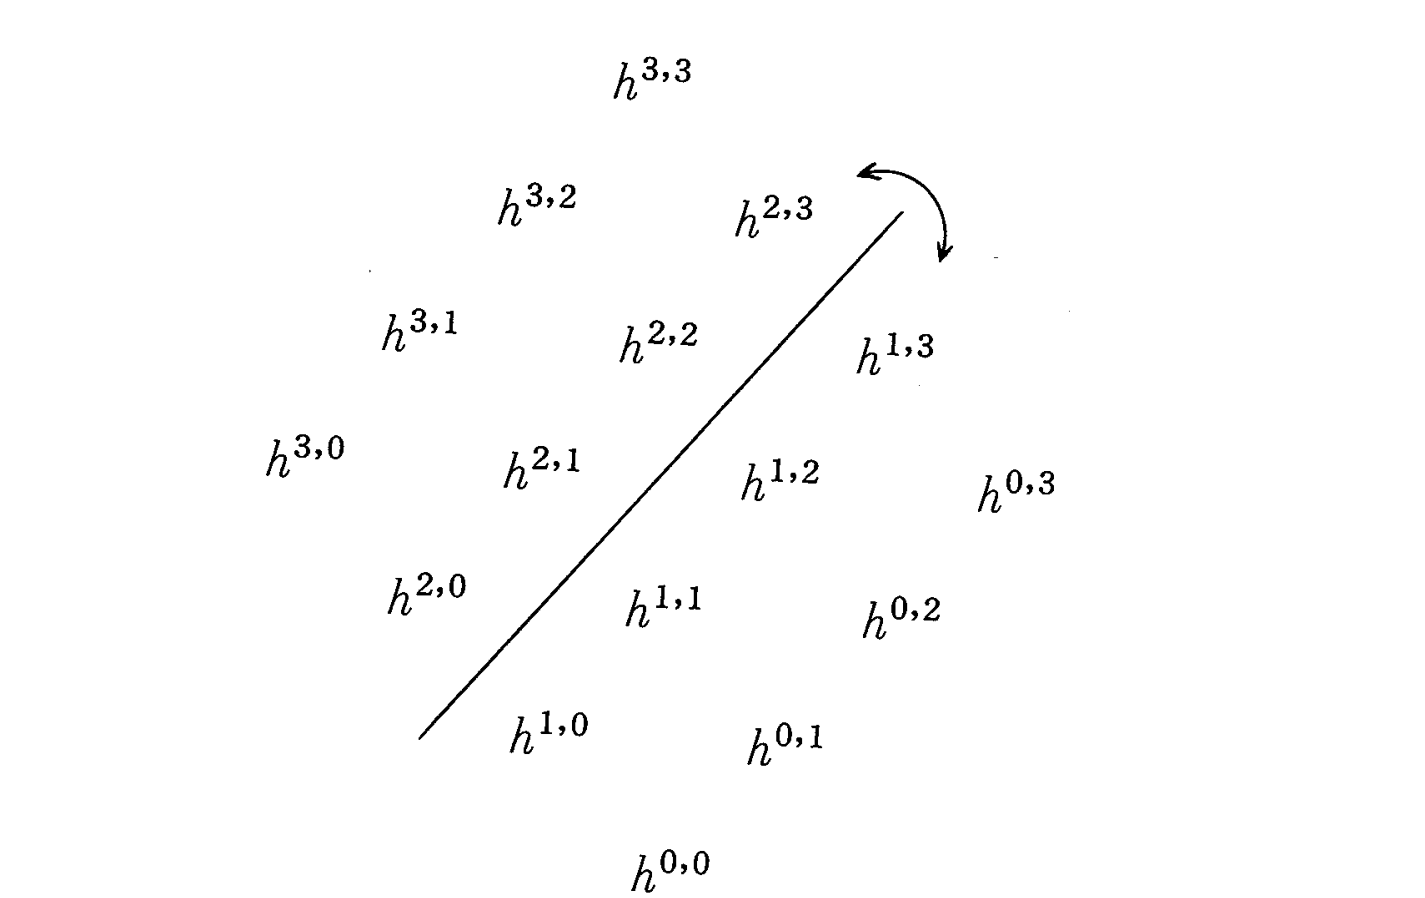
\includegraphics[width=0.62\textwidth]{figures/fig6.1.png}
  \figtitle{6.1}{霍奇菱形（原书 p.251）}
\end{figure}

$n=3$ 且 $H^1(M;\Q)=0$ 时，霍奇数全由 $h^{1,1}(M)$ 与 $h^{2,1}(M)$ 决定；此时 (6.7) 意味着 $h^{1,1}(M)=h^{2,1}(M^\dagger)$。
\end{remark}

\section{Gromov–Witten 不变量}

\takeaway{本节把 A 模型的量子杯积 $m_2^A$ 精确化，并推广到带标号点的一般黎曼面：用伪全纯曲线的模空间与求值映射定义 Gromov–Witten 类，从而得到量子上同调。}

本节的目的是把前一节概述过的 A 模型中的 $m_2^A$、即量子杯积的定义讲得更准确一些，并进一步加以推广。由前一节的定义 6.15 也可看出，$m_2^A$ 是利用伪全纯曲线的模空间给出的对应。考虑更一般的黎曼面，就能得到更多的映射。

从带标号点的黎曼面的模空间的考察开始。设 $\Sigma_g$ 为亏格 $g$ 的可定向 2 维流形。不固定 $\Sigma_g$ 上的复结构，只把它看作微分流形。
\[
  \mathfrak{J}(\Sigma_g)=\{J_{\Sigma_g}\mid\Sigma_g\text{ 上的光滑复结构}\}
\]
% [原文 p.252]
再设 $k$ 为 0 以上的整数，$z_1,\dots,z_k$ 为 $\Sigma_g$ 上相异的 $k$ 个点。合起来记作 $\vec z$。
\[
  \operatorname{Diff}(\Sigma_g,\vec z)=\{\psi\colon\Sigma_g\to\Sigma_g\mid\psi(z_i)=z_i,\ \psi\text{ 是微分同胚}\}
\]
$\operatorname{Diff}(\Sigma_g,\vec z)$ 作用于 $\mathfrak{J}(\Sigma_g)$。把这个作用的商空间记为 $\mathcal{M}_{g,k}=\mathfrak{J}(\Sigma_g)/\operatorname{Diff}(\Sigma_g,\vec z)$（$g$ 是亏格，$k$ 是所取点的个数）。$\mathfrak{J}(\Sigma_g)$ 赋予 $C^\infty$ 收敛的拓扑，$\mathcal{M}_{g,k}$ 的拓扑取为相应的商拓扑。以后省略 $\Sigma$ 的下标 $g$。
% [Tutor Note: 商空间 $\mathcal{M}_{g,k}$ 是轨形而非流形：$\operatorname{Diff}(\Sigma_g,\vec z)$ 在复结构上的作用有非平凡稳定化子（即 $(\Sigma,\vec z)$ 的自同构），定理 6.23 中的“轨形”正是指这一点。]

亏格为 $g$ 的黎曼面 $\Sigma$ 与其上相异的 $k$ 个点的组 $\vec z$ 给出 $\mathcal{M}_{g,k}$ 的一个元素。（说到黎曼面，就认为其上的复结构已确定。）$(\Sigma,\vec z)$ 与 $(\Sigma',\vec z')$ 给出同一元素，是指存在正纯同型 $\psi\colon\Sigma\to\Sigma'$ 使 $\psi(z_i)=z'_i$。这样的 $\psi$ 称为正纯同型 $(\Sigma,\vec z)\to(\Sigma',\vec z')$。

称 $(\Sigma,\vec z)$ 为\textbf{亏格 $g$ 带 $k$ 个标号点的黎曼面}（Riemann surface of genus $g$ with $k$ marked points）。$\mathcal{M}_{g,k}$ 是亏格 $g$ 带 $k$ 个标号点的黎曼面的正纯同型类全体。也写作 $(\Sigma,\vec z)\in\mathcal{M}_{g,k}$。

\begin{theorem}{6.23}
  若 $2g+k\geq3$，则 $\mathcal{M}_{g,k}$ 是（实）$6g-6+2k$ 维的轨形。
\end{theorem}

发现 $6g-6$ 这一维数的是 Riemann。定理 6.23 是复结构形变理论最基本的例子。大概会在 [371] 中解说，故此处说明从简。因为用到了轨形\footnote{引入轨形的是 Satake [323]，佐武称之为 V 流形（V-manifold）。orbifold 是其后很久 Thurston 使用的术语，如今后者似乎更为通行。最早把轨形用于代数曲线模空间研究的是 Mumford [272]。}一词，下面加以说明。

\begin{definition}{6.24}
  拓扑空间 $X$ 上的\textbf{轨形}（orbifold）结构，是指：开覆盖 $\bigcup U_i=X$；有限群 $\Gamma_i\subset GL(n;\R)$；$\R^n$ 中被 $\Gamma_i$ 的线性作用保持的开集 $V_i$；同胚 $\varphi_i\colon V_i/\Gamma_i\to U_i$；并且坐标变换都是微分同胚。

  若 $n=2n'$ 为偶数，$\Gamma_i\subset GL(n';\C)\subset GL(n;\R)$，且坐标变换都是正纯映射，则称之为\textbf{复轨形}。
\end{definition}

% [原文 p.253]
严格说应当定义“坐标变换是微分同胚”这句话，但很容易，故从略。

下面说明条件 $2g+k\geq3$ 的含义。对 $(\Sigma,\vec z)\in\mathcal{M}_{g,k}$，如下定义自同构群 $\operatorname{Aut}(\Sigma,\vec z)$。
\begin{equation}
  \operatorname{Aut}(\Sigma,\vec z)=\{\psi\colon\Sigma\to\Sigma\mid\psi\text{ 是双正纯},\ \psi(z_i)=z_i\}. \tag{6.8}
\end{equation}

\begin{lemma}{6.25}
  $2g+k\geq3$ 与 $\operatorname{Aut}(\Sigma,\vec z)$ 是有限群是等价的。
\end{lemma}

若 $g=0$、$k=0,1,2$，则 $\operatorname{Aut}(\Sigma,\vec z)$ 是 $\mathrm{PSL}(2;\C)$、即 $z\mapsto az+b$ 这样的变换全体 $\C^*$。又若 $g=1$、$k=0$，则 $\operatorname{Aut}(\Sigma,\vec z)$ 是环面。这些都是无限群。当 $2g+k\geq3$ 时 $\operatorname{Aut}(\Sigma,\vec z)$ 为有限群，其证明从略。

当紧 Lie 群 $G$ 作用于流形 $X$ 时，若对任意 $p\in X$，固定 $p$ 的 $G$ 的元素全体 $G_p$ 都是有限群，则商空间 $X/G$ 是轨形。

由于 $\mathfrak{J}(\Sigma_g)$、$\operatorname{Diff}(\Sigma_g,\vec z)$ 是无限维的，由引理 6.25 与上述注意，并不能直接证明定理 6.23 的前半部分、即 $\mathcal{M}_{g,k}$ 是轨形；但此处不再多作说明。定理 6.23 的维数计算可用 Riemann–Roch 定理作出。

\begin{remark}{6.26}
  $g=1$、$k=0$ 的情形是椭圆曲线的模空间，基本而且重要，但在定理 6.23 中被排除在外。$\operatorname{Aut}(T^2)$ 不是有限群，但其连通分支是 $T^2$ 自身，特别地紧。又 $\operatorname{Aut}(T^2)$ 的维数不依赖 $T^2$ 上的复结构。由此 $\mathcal{M}_{1,0}$ 仍然是轨形。只不过维数是 2，而不是 $6\cdot1-6=0$。
\end{remark}

$\mathcal{M}_{g,k}$ 的紧化 $C\mathcal{M}_{g,k}$ 很重要，但此处只引入这个记号，说明稍后再作。

其次，取 $M$ 为辛流形，并选好与 $\omega_M$ 相容的近复结构 $J_M$。设 $\beta\in H_2(M;\Z)$。令
% [原文 p.254]
\begin{equation}
  \begin{aligned}
    \tilde{\mathcal{M}}_{g,k}(M,J_M;\beta)=\bigl\{(J_\Sigma,\varphi)\mid{}&\varphi\colon\Sigma\to M\text{ 是伪全纯 }(J_M\circ\rd\varphi=\rd\varphi\circ J_\Sigma),\\
    &J_\Sigma\in\mathfrak{J}(\Sigma),\ \varphi_*[\Sigma]=\beta\bigr\}.
  \end{aligned} \tag{6.9}
\end{equation}
群 $\operatorname{Diff}(\Sigma_g,\vec z)$ 作用于 $\tilde{\mathcal{M}}_{g,k}(M,J_M)$，作用为 $\psi\cdot(J_\Sigma,\varphi)=(\psi^*J_\Sigma,\varphi\circ\psi^{-1})$。把商空间记为 $\mathcal{M}_{g,k}(M,J_M;\beta)$。拓扑取 $C^\infty$ 拓扑的商拓扑。

给定亏格 $g$ 带 $k$ 个标号点的黎曼面 $(\Sigma,\vec z)$ 与伪全纯映射 $\varphi\colon\Sigma\to M$，就确定 $\mathcal{M}_{g,k}(M,J_M;\beta)$ 的一个元素（其中 $\beta=\varphi_*[\Sigma]$）。$(\Sigma,\vec z,\varphi)$ 与 $(\Sigma',\vec z',\varphi')$ 确定 $\mathcal{M}_{g,k}(M,J_M;\beta)$ 的同一元素，等价于存在双正纯同型 $\psi\colon(\Sigma,\vec z)\to(\Sigma',\vec z')$ 使 $\varphi'\circ\psi=\varphi$。以后写作 $(\Sigma,\vec z,\varphi)\in\mathcal{M}_{g,k}(M,J_M;\beta)$。

\begin{theorem}{6.27}
  $\mathcal{M}_{g,k}(M,J_M;\beta)$ 的虚拟维数是 $2(n+c^1(\beta)+3g+k-3)$。
\end{theorem}

\begin{proof}[略证]
  由第 2 章的讨论，计算虚拟维数需要：模空间 $\mathcal{M}_{g,k}(M,J_M;\beta)$ 的定义方程的线性化，以及由群 $\operatorname{Diff}(\Sigma,\vec z)$ 的作用决定的椭圆型复形。（第 2 章没有写群的事情，参见 [126] 等。）当 $k=0$ 时，所求的椭圆型复形是 (6.10)。
  \begin{equation}
    T\Sigma\longrightarrow(T^{1,0}\Sigma\otimes\Lambda^{0,1}\Sigma)\oplus\varphi^*TM\longrightarrow\varphi^*TM\otimes\Lambda^{0,1}\Sigma. \tag{6.10}
  \end{equation}
  简单说明一下。$T\Sigma$ 的截面全体是 $\operatorname{Diff}(\Sigma)$ 的 Lie 代数。$T^{1,0}\Sigma\otimes\Lambda^{0,1}\Sigma$ 是 $\mathfrak{J}(\Sigma)$ 的切空间，$\varphi^*TM$ 是从 $\Sigma$ 到 $M$ 的映射全体的空间的切空间。$\varphi^*TM\otimes\Lambda^{0,1}\Sigma$ 是定义方程 $\rd\varphi\circ J_\Sigma-J_M\circ\rd\varphi=0$ 左边取值的地方。

  定义 (6.10) 的映射并计算其指数，留给读者。$\mathcal{M}_{g,k}(M,J_M;\beta)$ 的虚拟维数是 (6.10) 的指数变号后，再加上点的活动自由度 $2k$。
\end{proof}

对 $[\Sigma,\vec z,\varphi]\in\mathcal{M}_{g,k}(M,J_M;\beta)$，令 $\operatorname{ev}([\Sigma,\vec z,\varphi])=(\varphi(z_1),\dots,\varphi(z_k))\in M^k$，称之为\textbf{代入映射}（evaluation map）。$\operatorname{ev}$ 的第 $i$ 个成分记作 $\operatorname{ev}_i$。

\par\medskip\noindent\textbf{假定理 6.28}\ $\mathcal{M}_{g,k}(M,J_M;\beta)$ 被紧化到光滑闭流形 $C\mathcal{M}_{g,k}(M,J_M;\beta)$，且 $\operatorname{ev}$ 可扩充为从 $C\mathcal{M}_{g,k}(M,J_M;\beta)$ 出发的光滑映射。\hfill$\square$\par\medskip

% [原文 p.255]
这个“定理”是假的。本节后面还会稍作说明（准确的定理见 [124] Chapter 4）。暂且承认 6.28 先往下走。

对 $[\Sigma,\vec z,\varphi]\in\mathcal{M}_{g,k}(M,J_M;\beta)$，确定 $[\Sigma,\vec z]\in\mathcal{M}_{g,k}$。把这个映射记为 $\mathrm{fg}\colon\mathcal{M}_{g,k}(M,J_M;\beta)\to\mathcal{M}_{g,k}$，称为\textbf{遗忘映射}（forgetting map）。$\mathrm{fg}$ 可扩充为 $\mathrm{fg}\colon C\mathcal{M}_{g,k}(M,J_M;\beta)\to C\mathcal{M}_{g,k}$（参见注意 6.60）。

\begin{definition}{6.29}
\[
  \resizebox{0.97\linewidth}{!}{$\displaystyle (\operatorname{ev},\mathrm{fg})_*[C\mathcal{M}_{g,k}(M,J_M;\beta)]\in H_{2(n+c^1(\beta)+3g+k-3)}(M^k\times C\mathcal{M}_{g,k};\Q) $}
\]
  称为\textbf{Gromov–Witten 不变量}（Gromov-Witten invariant），记作 $GW_{g,k}(M,\omega_M;\beta)$。
\end{definition}

\begin{theorem}{6.30}
  Gromov–Witten 不变量由 $M$ 的辛结构决定，不依赖相容的近复结构。
\end{theorem}

\begin{remark}{6.31}
  只看定义 6.29，Gromov–Witten 不变量似乎就是整数系数的同调类。这一点与 6.28 是假的相关，其说明本书从略。只写结论：下面 2 个条件中任一成立时，$GW_{0,k}(M,\omega_M;\beta)$ 是整数系数的同调类。
  \begin{enumerate}[label=(\arabic*),leftmargin=2.2em,itemsep=1pt,topsep=2pt]
    \item $(M,\omega_M)$ 是半正定的，且不存在 $\beta=d\beta'$、$\beta'\in H_2(M;\Z)$、$d$ 为 2 以上自然数的这样的 $d,\beta'$\footnote{$k\geq3$ 时，若 $(M,\omega_M)$ 半正定，则 $GW_{0,k}(M,\omega_M;\beta)$ 是整数系数的同调类（[319]）。}。
    \item 对任意满足 $\beta'\cap\omega_M>0$ 的 $\beta'\in H_2(M;\Z)$，都有 $c^1(\beta')>0$。（把这个条件称为\textbf{强正}（strongly positive）。单调则强正。）
  \end{enumerate}
  Calabi–Yau 流形的情形下 (2) 不成立，因此对 $\beta=d\beta'$，Gromov–Witten 不变量不是整数系数的同调类。另一方面，Calabi–Yau 流形是半正定的，Floer 同调是整数系数定义的。后面要叙述的量子上同调环也用整数系数定义。
\end{remark}

\begin{remark}{6.32}
  在定理 6.30、定义 6.29 中并未假设 $2g+k\geq3$。
\end{remark}
% [Tutor Note: 定义 6.29 的同调类取 $\Q$ 系数：紧化后的模空间一般只是轨形，须用虚拟基本类，未必有整数基本类；这正是“6.28 是假的”所指向的技术困难，注意 6.31 讨论的正是它。]

容易看出，$\mathcal{M}_{0,3}=C\mathcal{M}_{0,3}$ 是一个点。因此 $GW_{0,3}(M,\omega_M;\beta)$ 是 $H_{2(n+c^1(\beta))}(M^3;\Q)$ 的元素。用这个元素与斜积，§6.1 的 $m^A_{2,\beta}$ 可表示如下。
% [原文 p.256]
\[
  m^A_{2,\beta}(P,Q)=(P\times Q)/GW_{0,3}(M,\omega_M;\beta)
\]

这里回到前面，说明模空间的紧化。

先说明 $C\mathcal{M}_{g,k}$。要把满足给定条件的几何结构的同型类全体、即模空间紧化，一般原理是：把退化所产生的带奇点的结构也纳入考虑。带标号点的黎曼面的模空间的紧化，也是把带奇点的代数曲线\footnote{有奇点时就不称为黎曼面。}加进来作紧化。代数曲线的奇点有各种各样，但已知只允许最简单的奇点就足够了。即在 $\C^2$ 中局部同构于 $\C\times\{0\}\cup\{0\}\times\C$ 的奇点。称之为\textbf{通常二重点}（ordinary double point）。本书避免使用代数几何的知识，而如下定义。

\begin{definition}{6.33}
  紧 Hausdorff 空间 $\Sigma$ 上的\textbf{半稳定曲线}（semistable curve）结构，是指：由有限个互不相交的黎曼面之和 $\bigcup\Sigma_i$ 到 $\Sigma$ 的连续映射 $\pi\colon\bigcup\Sigma_i\to\Sigma$，且满足以下条件。
  \begin{enumerate}[label=(\arabic*),leftmargin=2.2em,itemsep=1pt,topsep=2pt]
    \item 存在有限集合 $S(\Sigma)\subset\Sigma$，使 $\pi$ 的限制 $\bigcup\Sigma_i-\pi^{-1}(S(\Sigma))\to\Sigma-S(\Sigma)$ 是同胚。
    \item 对 $p\in S(\Sigma)$，$\pi^{-1}(p)$ 恰好由 2 点组成。
  \end{enumerate}
  称 $S$ 的点为\textbf{奇点}（singular point），$\Sigma-S(\Sigma)$ 的点为\textbf{正则点}（regular point）。$\Sigma-S(\Sigma)$ 的连通分支的闭包称为 $\Sigma$ 的\textbf{既约成分}（irreducible component）。$\bigcup\Sigma_i$ 称为 $\Sigma$ 的\textbf{正规化}（normalization）。
\end{definition}

下面图 6.2 的 (a)、(b) 是半稳定曲线，而 (c)、(d) 不是半稳定曲线。以后为用语方便，也说 $\Sigma$ 是半稳定曲线等等。
% [Tutor Note: 条件 (2) 要求 $\pi^{-1}(p)$ 恰为 2 点，正对应“通常二重点”的两个分支；图 6.2 的 (c) 是三重点、(d) 有尖点，故都被排除。]

% [原文 p.257]
\begin{figure}[htbp]
  \centering
  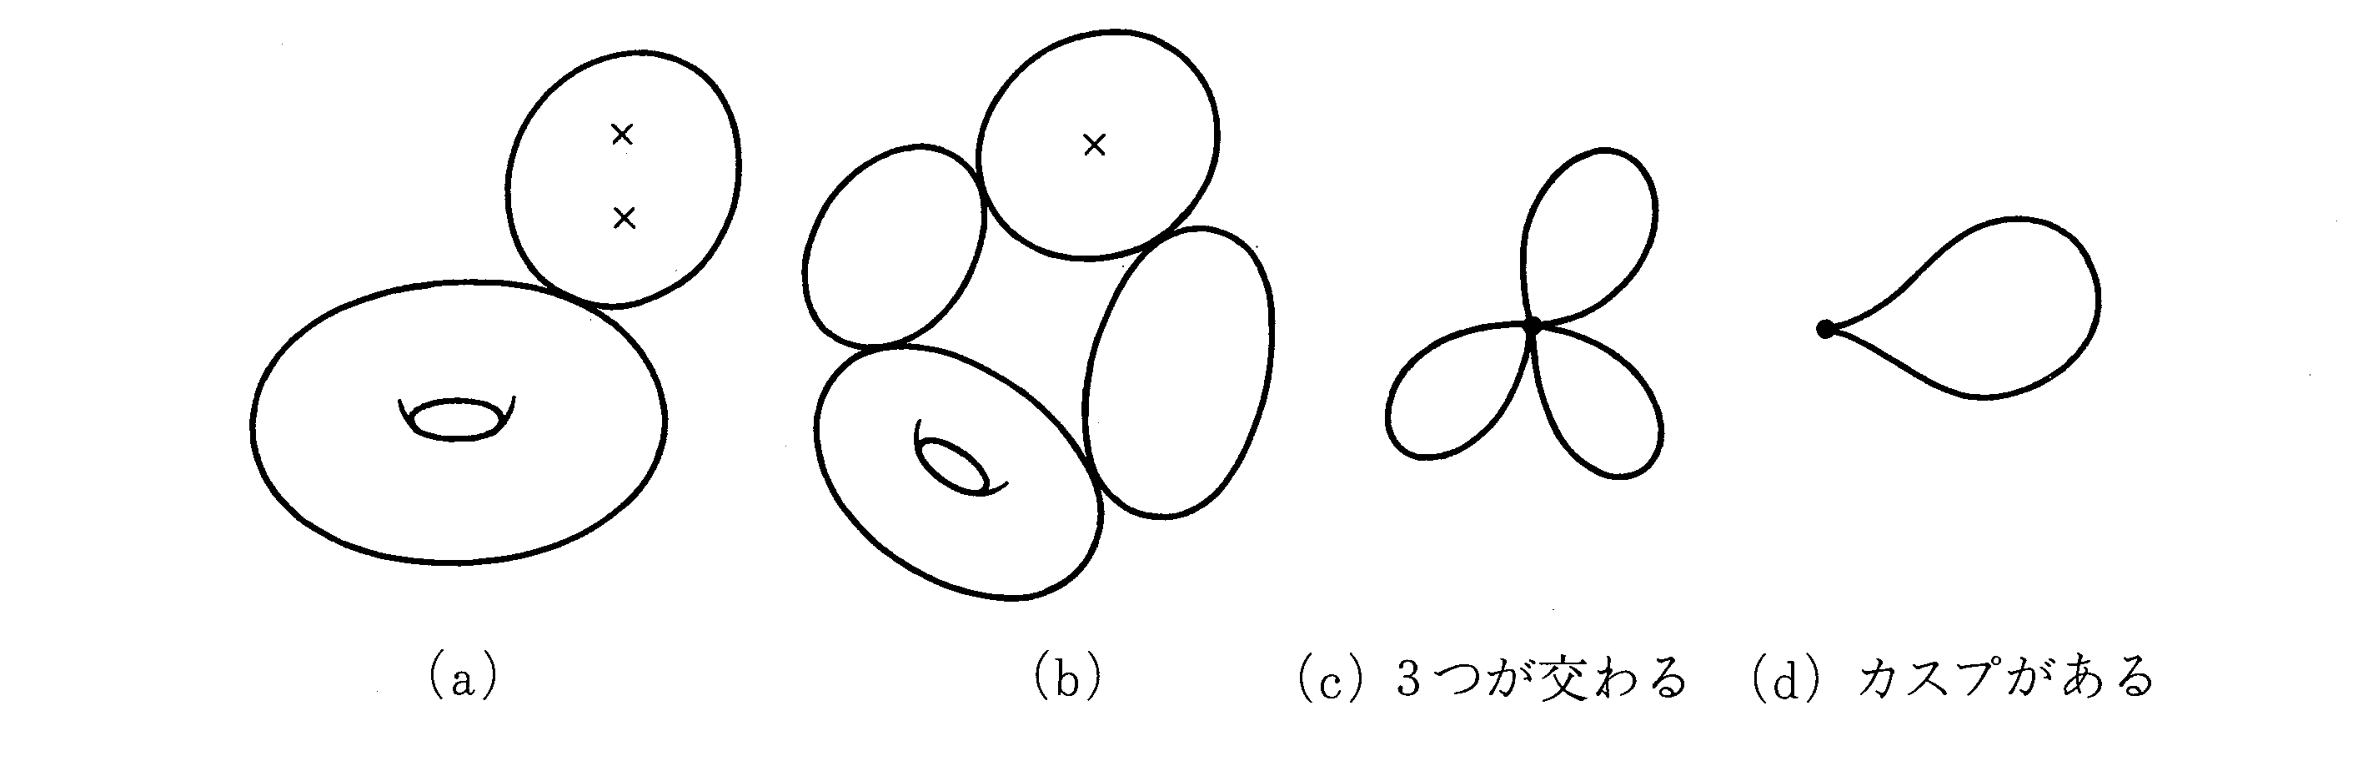
\includegraphics[width=0.92\textwidth]{figures/fig6.2.png}
  \figtitle{6.2}{半稳定曲线 (a)、(b) 与不是半稳定曲线的 (c)、(d)（原书 p.257）}
\end{figure}

设 $z_1,\dots,z_k$ 为 $\Sigma$ 的互不相同的正则点，此时称 $(\Sigma,\vec z)$ 为\textbf{$k$ 点付半稳定曲线}（$k$ pointed semistable curve）。

$\Sigma_i$ 们与 $\Sigma$ 的既约成分有时同构，但如图 6.2 的 (b) 那样，$\Sigma$ 的既约成分有自交时，这两者就不同。这是本书专用的术语：把 $\Sigma_i$ 们称为\textbf{非奇异既约成分}。

\begin{definition}{6.34}
  设 $\Sigma,\Sigma'$ 为半稳定曲线。同胚 $\psi\colon\Sigma\to\Sigma'$ 是\textbf{正纯同型}（biholomorphic map），是指存在正规化 $\bigcup\Sigma_i$ 与 $\bigcup\Sigma'_i$ 之间的正纯同型 $\tilde\psi\colon\bigcup\Sigma_i\to\bigcup\Sigma'_i$ 且它诱导 $\psi$。

  当 $\psi(z_i)=z'_i$ 时，称 $\psi$ 是带标号点半稳定曲线 $(\Sigma,\vec z),(\Sigma',\vec z')$ 之间的正纯同型。$(\Sigma,\vec z)$ 到自身的正纯同型全体构成群，记作 $\operatorname{Aut}(\Sigma,\vec z)$。
\end{definition}

对半稳定曲线 $\Sigma$，可以变形奇点而得到（非奇异的）黎曼面。$\Sigma$ 的亏格就是指所得黎曼面的亏格。图 6.2 的 (a)、(b) 的亏格分别是 1、2。下面准确给出亏格的定义。对半稳定曲线如下对应一个图 $\Gamma_\Sigma$。对 $\Sigma$ 的每个既约成分，对应 $\Gamma_\Sigma$ 的一个\textbf{顶点}（vertex）。又，对奇点对应 $\Gamma_\Sigma$ 的一条\textbf{边}（edge）。与 $p$ 对应的边的两端，接在与含 $\pi^{-1}(p)$ 的 2 个既约成分对应的 $\Gamma_\Sigma$ 的顶点上。（若 $\pi^{-1}(p)$ 的 2 点都含在 $\Sigma_i$ 中，则与 $\Sigma_i$ 对应的顶点上有一条两端都是该顶点的边。）在 $\Gamma_\Sigma$ 的顶点上写下对应既约成分的亏格 $g_i$。

带标号点半稳定曲线的情形，取个数为点数 $k$ 的边，把其一端分别接在与各点所属既约成分对应的顶点上。另一端不连接，而作为新的顶点。$k$ 点付半稳定曲线中既约成分的个数为 $m$ 时，顶点数为 $k+m$。在新添的顶点处写下它对应第几个点。

图 6.2 的 (a)、(b) 的带标号点半稳定曲线对应图 6.3 的图 (a)、(b)。
% [原文 p.258]
\begin{figure}[htbp]
  \centering
  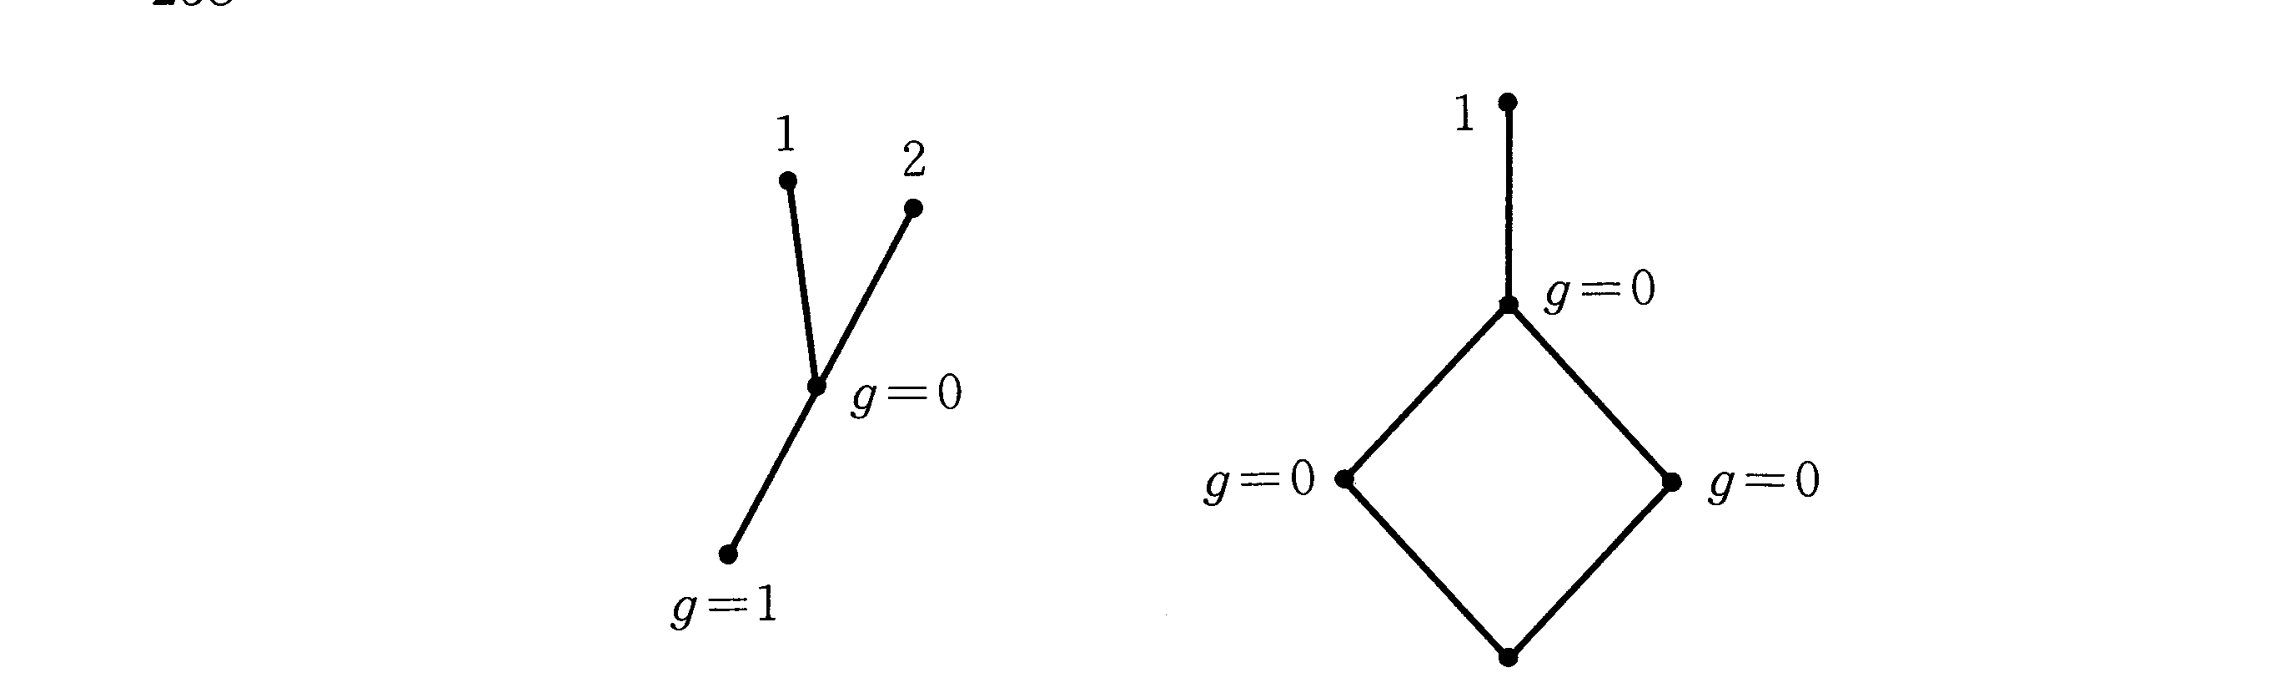
\includegraphics[width=0.92\textwidth]{figures/fig6.3.png}
  \figtitle{6.3}{图（原书 p.258）}
\end{figure}

\begin{definition}{6.35}
  称 $\sum g_i+\operatorname{rank}H_1(\Gamma_\Sigma;\Q)$ 为半稳定曲线 $\Sigma$ 的\textbf{亏格}（genus）。
\end{definition}

若为紧化 $\mathcal{M}_{g,k}$ 而把半稳定曲线的正纯同型类全体都加进去，所得空间就不是 Hausdorff 空间，得不到正确的紧化。

\begin{example}{6.36}
  考虑图 6.4(a) 的半稳定曲线 $\Sigma$。把 $\Sigma$ 在奇点附近变形，就得到图 6.4(b) 的 $\Sigma'$，但图 6.4(b) 不论把粘合的颈部弄得多细，都表示同一个半稳定曲线。即 $\lim_{i\to\infty}\Sigma^i=\Sigma$\footnote{不明确极限的意义，这个式子就没有意义。拓扑的定义见 [124] §10。}。这里左边指对任何 $i\in\Z$ 都取 $\Sigma^i$ 的列的极限。另一方面 $\lim_{i\to\infty}\Sigma^i=\Sigma'$，故模空间不是 Hausdorff 空间。这一现象的根源在于 $\Sigma$ 的自同构群 $\operatorname{Aut}(\Sigma')$ 不紧。$\operatorname{Aut}(\Sigma')$ 含有左端既约成分的自同构（形如 $z\mapsto az+b$ 的映射 $\CP^1\to\CP^1$ 全体）。这个群的作用消去了把颈部越弄越细的自由度，于是发生了 $\lim_{i\to\infty}\Sigma^i=\Sigma$ 这样的事。
\end{example}

我们已经在第 3 章遇到过同样的现象。即，考虑非紧复 Lie 群作成的商 $X/G_\C$ 时，若不只取 $X$ 全体而只取稳定元，商空间就不是 Hausdorff 空间。

% [原文 p.259]
\begin{figure}[htbp]
  \centering
  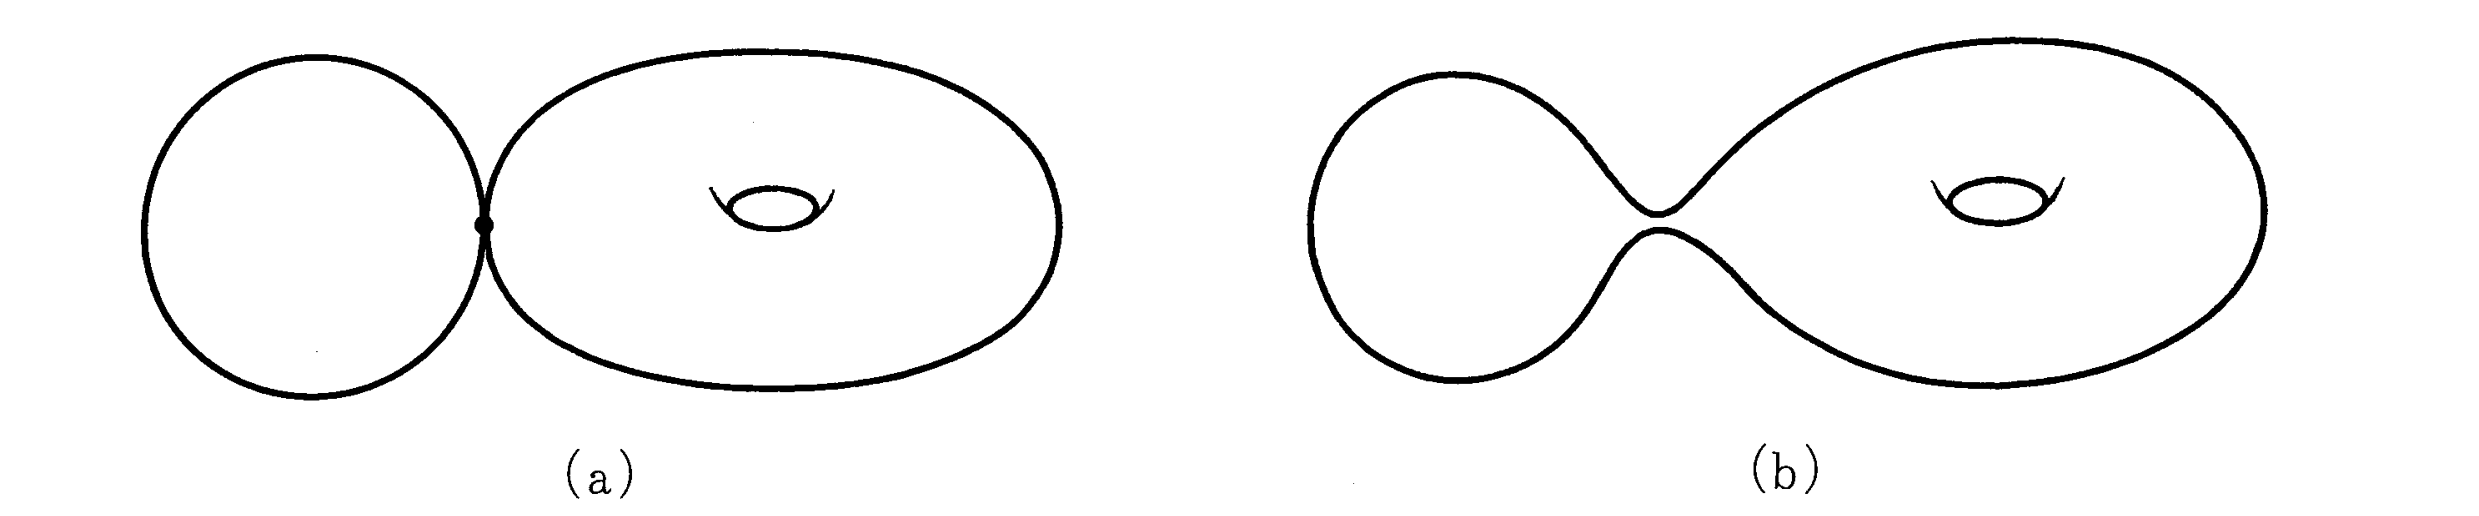
\includegraphics[width=0.9\textwidth]{figures/fig6.4.png}
  \figtitle{6.4}{非 Hausdorff（原书 p.259）}
\end{figure}

在我们的情形，商空间 $\mathfrak{J}(\Sigma_g)/\operatorname{Diff}(\Sigma_g,\vec z)$ 本身是 Hausdorff 空间。也就是说，Hausdorff 性只在无穷远处崩坏。这一点上情况略有不同，但本质上需要同样的想法。来定义稳定性。

\begin{definition}{6.37}
  带标号点半稳定曲线 $(\Sigma,\vec z)$ 是\textbf{稳定}（stable）的，是指自同构群 $\operatorname{Aut}(\Sigma,\vec z)$ 是有限群。
\end{definition}

用引理 6.25 可以判定稳定性。对 $(\Sigma,\vec z)$ 的非奇异既约成分 $\Sigma_i$，把 $\pi^{-1}(S)\cap\Sigma_i$ 的元素称为它的\textbf{奇点}（singular point），把 $\pi^{-1}\{z_1,\dots,z_k\}\cap S$ 的点称为\textbf{带名点}（marked point）。奇点或带名点统称为\textbf{特殊点}（special point）。

\begin{lemma}{6.38}
  $(\Sigma,\vec z)$ 稳定，等价于下述条件：设非奇异既约成分 $\Sigma_i$ 的亏格为 $g_i$、特殊点的个数为 $k_i$，则对任意 $i$ 都有 $2g_i+k_i\geq3$。
\end{lemma}

证明由引理 6.25 显然。现在假设 $2g+k\geq3$。把亏格 $g$ 的 $k$ 点付稳定曲线的正纯同型类全体记为 $C\mathcal{M}_{g,k}$。

\begin{theorem}{6.39}（Deligne–Mumford [69]）
  $C\mathcal{M}_{g,k}$ 上确定复轨形的结构。
\end{theorem}

往 $C\mathcal{M}_{g,k}$ 上放入复轨形结构的方法，参见 [124] §9、[371] §4.1。

\begin{example}{6.40}
  $\mathcal{M}_{0,4}$ 是 $\CP^1$ 上相异的 4 点 $(z_1,z_2,z_3,z_4)$ 的组全体的集合，用 $\CP^1$ 的自同构即 $PSL(2;\C)$ 的作用取的商空间。如所周知，对 $\CP^1$ 上相异的 3 点，存在唯一的 $PSL(2;\C)$ 元素把它们移到 $0,1,\infty$。故 $\mathcal{M}_{0,4}$ 是 $\CP^1-\{0,1,\infty\}$。要把它紧化，加上 $\{0,1,\infty\}$ 即可。所加的
\end{example}

% [原文 p.260]
\begin{figure}[htbp]
  \centering
  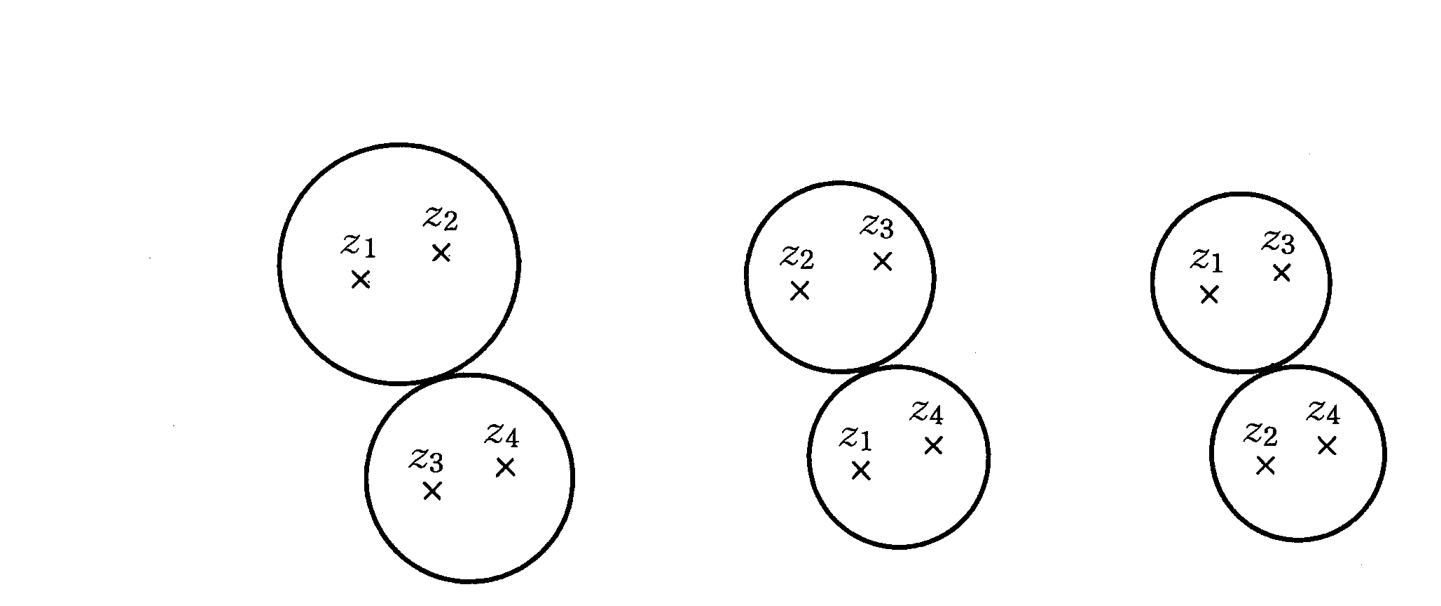
\includegraphics[width=0.82\textwidth]{figures/fig6.5.png}
  \figtitle{6.5}{$\mathcal{M}_{0,4}$ 的无穷远点（原书 p.260）}
\end{figure}

$C\mathcal{M}_{0,4}-\mathcal{M}_{0,4}$ 的元素分别对应图 6.5 的半稳定曲线。

\begin{example}{6.41}
  $\mathcal{M}_{0,5}$ 是实 4 维的。紧化时加进来的，首先是图 6.6 那样的半稳定曲线的族 $C_{i,j}\subset C\mathcal{M}_{0,5}$。这种取法是从 5 个数中选 2 个的选法，故有 10 种。它们分别与 $\mathcal{M}_{0,4}$、即 $\CP^1-\{0,1,\infty\}$ 复同构。

  $C_{i,j}$ 在 $C\mathcal{M}_{0,5}$ 中的闭包记为 $\bar C_{i,j}$。$\bar C_{i,j}$ 与 $\CP^1$ 同构。$\bar C_{i,j}-C_{i,j}$ 是 3 点。把它们全部合起来，得到 $3\times10/2=15$ 个点。这 15 个点所表示的半稳定曲线 $\Sigma$ 与对应的图 $\Gamma_\Sigma$ 一一对应。
\end{example}

\begin{figure}[htbp]
  \centering
  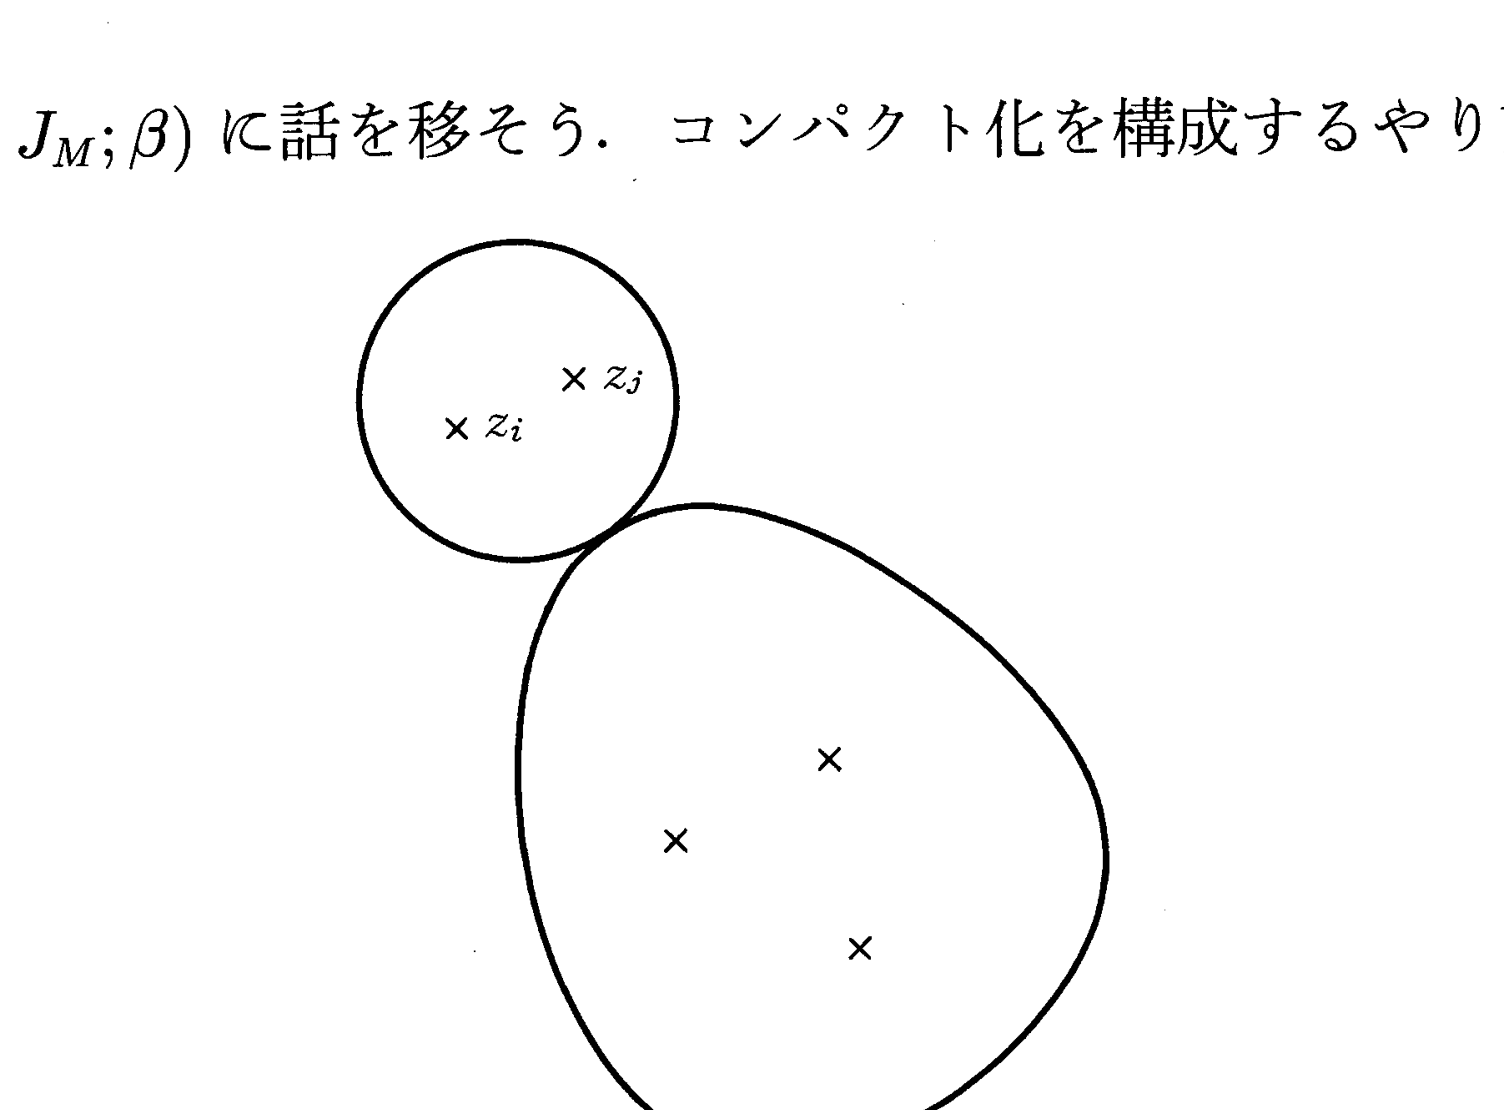
\includegraphics[width=0.56\textwidth]{figures/fig6.6.png}
  \figtitle{6.6}{$\mathcal{M}_{0,5}$ 的无穷远点（原书 p.260）}
\end{figure}

转到 $C\mathcal{M}_{g,k}(M,J_M;\beta)$。构成紧化的方式基本上与 $C\mathcal{M}_{g,k}$ 的情形相同，要点之一是适当的稳定性定义。

% CHUNK ch06a DONE
